\documentclass{article}
\usepackage{graphicx} 
\usepackage{float}
\usepackage{gensymb}
\usepackage{amsmath}
\usepackage{listings}
\usepackage{amssymb}
\usepackage[paperheight=6in,
   paperwidth=5in,
   top=10mm,
   bottom=20mm,
   left=15mm,
   right=15mm]{geometry}
\usepackage{lipsum}
\usepackage{graphicx} 
\usepackage{tikz}
\usetikzlibrary{calc}
\begin{document}
\begin{center}
   \textbf{MATLAB assignment-2}\\
   Pritha Jana,IMS21276
    \end{center}
\bigskip
\begin{enumerate}
    \item \textbf{Question-1:} Write MATLAB script to implement the Euler’s method to solve the initial value problems
(IVPs) given below $\frac{dy}{dx}$=$y-x$ and $y(0) = 0.5$,
with $h=0.1$ and $h=0.05$ to obtain the approximation to $y(1)$. Given that the exact solution to the IVP is $y(x) = x+1-0.5e^x$.Plot the solutions with the step-sizes $h = 0.1$ and $h = 0.05$,what do you observe? Explain the behavior.Compare the errors at two approximations to $y(1)$.\\
\textbf{Answer:}\\
\textbf{Code:}\\
\underline{For $h=0.1$}
    \begin{lstlisting}
clear all;
close all;
format short 
h=0.1;
x=0:h:1;
N=length(x)
y(1)=0.5;
f=@(x,y) y-x;
ye=@(x) x+1-0.5.*exp(x);
for i=1:N-1;
    y(i+1)=y(i)+h*f(x(i),y(i))
end
exactsol=ye(x);
error=max(abs(y-ye(x)))
plot(x,y,'-*',x,exactsol,'r')

\end{lstlisting}
\textbf{Result:}
\begin{lstlisting}
    y =
    0.5000    0.5500    0.5950    0.6345    0.6680    0.6947    0.7142    0.7256    0.7282    0.7210    0.7031
    error =0.0623
\end{lstlisting}
\textbf{Figure:}
\begin{figure}[H]                                 
	  \centering                          
	  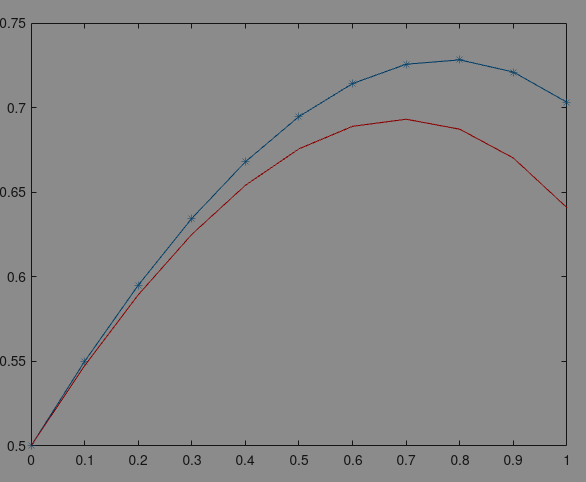
\includegraphics[width=\columnwidth]{fig1.png}
\caption{}
\label{fig:1.1}                        
  \end{figure}
\underline{For $h=0.05$}
\begin{lstlisting}
% Question- 1)b)
clear all;
close all;
format short 
h=0.05;
x=0:h:1;
N=length(x)
y(1)=0.5;
f=@(x,y) y-x;
ye=@(x) x+1-0.5.*exp(x);
for i=1:N-1;
    y(i+1)=y(i)+h*f(x(i),y(i))
end
exactsol=ye(x);
error=max(abs(y-ye(x)))
plot(x,y,'-*',x,exactsol,'r')

\end{lstlisting}
\textbf{Result:}
\begin{lstlisting}
0.7040    0.6967    0.6865    0.6734
error =0.0325
\end{lstlisting}
\textbf{Figure:}
\begin{figure}[H]                                 
	  \centering                          
	  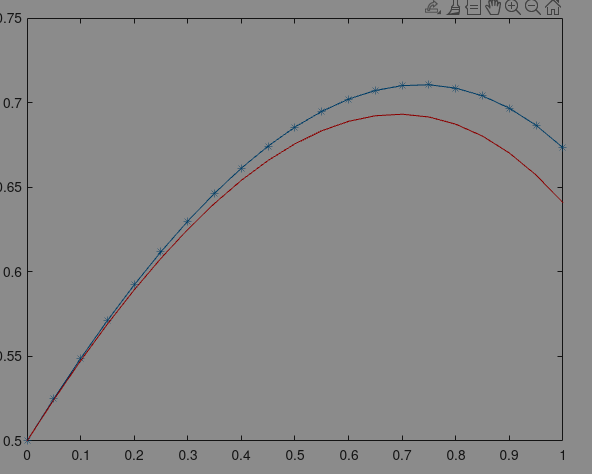
\includegraphics[width=\columnwidth]{fig2.png}
\caption{}
\label{fig:1.1}                        
  \end{figure}
\textbf{Observations:}As the value of $h$ decreases the error become less so the difference approximated curve and the exact curve become less.
\item \textbf{Question-2:}Write Matlab code for the modified Euler’s method $y_j+1 = y_j+\frac{h}{2}(f(x_j,y_j)+f(x_j+1, y_j+1)),j=1, 2, . . .$ for the above IVP with $h = 0.1$ to obtain the approximation to $y(1)$. Compare results with
forward and backward Euler’s method.\\
\textbf{Answer:}\\
\textbf{Code:}\\
\begin{lstlisting}
% Question-2)
clear all;
close all;
format short 
h=0.1;
x=0:h:1;
N=length(x);
y(1)=0.5;
f=@(x,y) y-x;
ye=@(x) x+1-0.5.*exp(x);
for i=1:N-1;
    y(i+1)=(y(i)+(h/2)*(f(x(i),y(i))-x(i+1)))/(1-(h/2))
end
exactsol=ye(x);
error=max(abs(y-ye(x)))
plot(x,y,'-*',x,exactsol,'r')

\end{lstlisting}
\textbf{Result:}
\begin{lstlisting}
y =
0.5000    0.5474    0.5892    0.6249    0.6538    0.6753    0.6885    0.6925    0.6865    0.6693    0.6397
error =0.0011
\end{lstlisting}
\textbf{Observations:} Forward difference giving us error 0.0325 and Backward difference giving us 0.0748 and the modified Euler's method giving us error 0.0011. So,we are getting best result for modified one.\\
\textbf{Figure:}
\begin{figure}[H]                                 
	  \centering                          
	  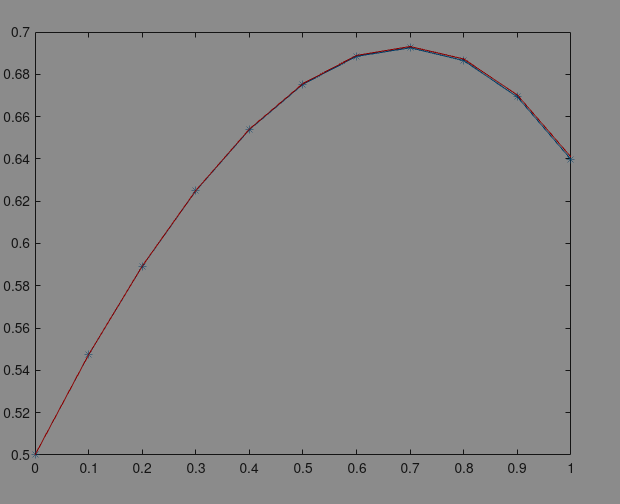
\includegraphics[width=\columnwidth]{fig3.png}
\caption{}
\label{fig:1.1}                        
  \end{figure}
\item \textbf{Question-3:}Write MATLAB script to implement the Runge-Kutta (RK) methods of order 2, 3 and order4 to solve the above given IVPs.\\
\textbf{Answer:}\\
\textbf{Code:}\\
\underline{RK methods of order 2}
\begin{lstlisting}
%Questin-3)
%RK methods of order 2
clear all;
close all;
format short 
h=0.1;
x=0:h:1;
N=length(x)
y(1)=0.5;
f=@(x,y) y-x;
ye=@(x) x+1-0.5.*exp(x);
for i=1:N-1;
    k1=h*(f(x(i),y(i)));
    k2=h*(f((x(i)+(1/2)),(y(i)+(k1/2))));
    k3=h*(f((x(i)+(h/2)),(y(i)+(k2/2))));
    k4=h*f((x(i)+h),(y(i)+k3));
    y(i+1)=(y(i))+h*(1/2)*(k1+k2)
end
exactsol=ye(x);
error=max(abs(y-ye(x)))
plot(x,y,'-*',x,exactsol,'r')
\end{lstlisting}
\textbf{Result:}
\begin{lstlisting}
y =
 0.5000    0.5026    0.5043    0.5049    0.5045    0.5030    0.5006    0.4971    0.4925    0.4868    0.4801
error =0.1961
\end{lstlisting}
\textbf{Figure:}
\begin{figure}[H]                                 
	  \centering                          
	  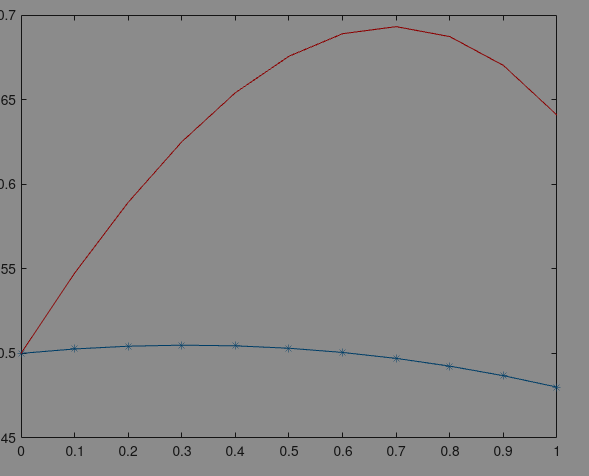
\includegraphics[width=\columnwidth]{fig4.png}
\caption{}
\label{fig:1.1}                        
  \end{figure}
\underline{RK methods of order 3}
\begin{lstlisting}
%RK methods of order 3
clear all;
close all;
format short 
h=0.1;
x=0:h:1;
N=length(x)
y(1)=0.5;
f=@(x,y) y-x;
ye=@(x) x+1-0.5.*exp(x);
for i=1:N-1;
    k1=h*(f(x(i),y(i)));
    k2=h*(f((x(i)+(1/2)),(y(i)+(k1/2))));
    k3=h*(f((x(i)+(h/2)),(y(i)+(k2/2))));
    k4=h*f((x(i)+h),(y(i)+k3));
   y(i+1)=(y(i))+(h/6)*(k1+(4*k2)+k3)
end
exactsol=ye(x);
error=max(abs(y-ye(x)))
plot(x,y,'-*',x,exactsol,'r')

\end{lstlisting}
\textbf{Result:}
\begin{lstlisting}
y = 0.5000    0.5018    0.5025    0.5022    0.5008    0.4984    0.4949    0.4904    0.4847    0.4780    0.4701
error = 0.2027
\end{lstlisting}
\textbf{Figure:}
\begin{figure}[H]                                 
	  \centering                          
	  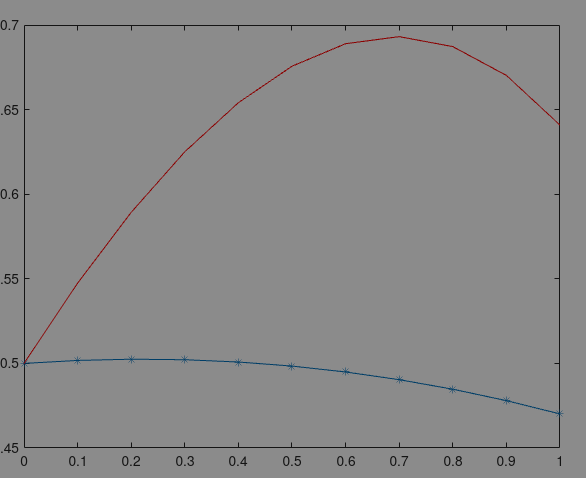
\includegraphics[width=\columnwidth]{fig5.png}
\caption{}
\label{fig:1.1}                        
  \end{figure}

  \underline{RK methods of order 3}
\begin{lstlisting}
%RK methods of order 4
clear all;
close all;
format short 
h=0.1;
x=0:h:1;
N=length(x)
y(1)=0.5;
f=@(x,y) y-x;
ye=@(x) x+1-0.5.*exp(x);
for i=1:N-1;
    k1=h*(f(x(i),y(i)));
    k2=h*(f((x(i)+(1/2)),(y(i)+(k1/2))));
    k3=h*(f((x(i)+(h/2)),(y(i)+(k2/2))));
    k4=h*f((x(i)+h),(y(i)+k3));
    y(i+1)=(y(i))+(1/6)*(k1+(2*k2)+(2*k3)+k4)
end
exactsol=ye(x);
error=max(abs(y-ye(x)))
plot(x,y,'-*',x,exactsol,'r')

\end{lstlisting}
\textbf{Result:}
\begin{lstlisting}
y = 0.5000    0.5316    0.5561    0.5726    0.5803    0.5783    0.5655    0.5409    0.5033    0.4511    0.3829
error = 0.2579
\end{lstlisting}
\textbf{Figure:}
\begin{figure}[H]                                 
	  \centering                          
	  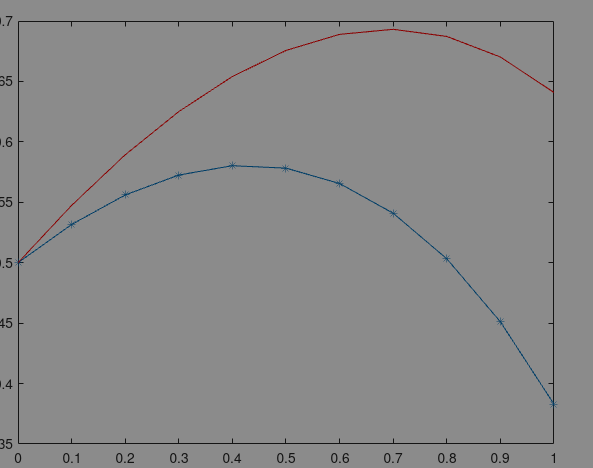
\includegraphics[width=\columnwidth]{fig6.png}
\caption{}
\label{fig:1.1}                        
  \end{figure}
\item \textbf{Question-4:}Run the Euler and RK methods codes for different h and find the order of convergence for
each rule. Write down your observation.\\
\textbf{Answer:}\\
\textbf{Code:}\\
\underline{For Euler Method}
\begin{lstlisting}
% Question-4)
%Euler Method
clear all
close all;
format long
for lel=1:4
h=1*10^(-lel);
H(lel)=h;
x=0:h:1;
N=length(x);
y(1)=0.5; 
f=@(x,y)  y-x;
ye=@(x)  x+1-0.5.*exp(x);
for i=1:N-1;
    y(i+1)=y(i)+h*f(x(i),y(i));
end

exactsol=ye(x);
error(lel)=max(abs(y-exactsol))
end

for k=1:lel-1
ordercg(k)=log(error(k)/error(k+1))/log(H(k)/H(k+1))
end
loglog(H,error,'-*')
\end{lstlisting}
\textbf{Result:}
\begin{lstlisting}
error = 0.062269684179523   0.006733999518759   0.000678948111575   0.000067950816917
ordercg = 0.966003582049147   0.996436496304685   0.999641902443317
\end{lstlisting}
\underline{For RK methods of order 4}
\begin{lstlisting}
%Rk Method
clear all
close all;
format long
for lel=1:4
h=1*10^(-lel);
H(lel)=h;
x=0:h:1;
N=length(x);
y(1)=0.5; 
f=@(x,y)  y-x;
ye=@(x)  x+1-0.5.*exp(x);
for i=1:N-1;
    k1=h*(f(x(i),y(i)));
    k2=h*(f((x(i)+(1/2)),(y(i)+(k1/2))));
    k3=h*(f((x(i)+(h/2)),(y(i)+(k2/2))));
    k4=h*f((x(i)+h),(y(i)+k3));
    y(i+1)=(y(i))+(1/6)*(k1+(2*k2)+(2*k3)+k4);
end

exactsol=ye(x);
error(lel)=max(abs(y-exactsol))
end

for k=1:lel-1
ordercg(k)=log(error(k)/error(k+1))/log(H(k)/H(k+1))
end
loglog(H,error,'-*')

\end{lstlisting}
\textbf{Result:}
\begin{lstlisting}
error =0.257934933058065   0.283518840636149   0.286093948255741   0.286351666951306
ordercg = -0.041071760106760  -0.003926746977085  -0.000391044361090
\end{lstlisting}
\textbf{Observations:}Euler method is compatible for the above problem with order of convergence of $o(h)$. But the RK method for order of 4 is incompatible for the problem as it is giving negative convergence for smaller value of $h$. 
\item \textbf{Question-5:}Write Forward Euler and RK 2 code for system of equations, solve following PDE using that $y'' + 2xy'-x^2y=0, y(0)=2, y'(0)=-1.$\\
\textbf{Answer:}\\
\textbf{Code:}\\
\underline{Forward Euler method}
\begin{lstlisting}
%Question-5)
clear all;
close all;
format short 
h=0.1;
x=0:h:1;
N=length(x);
y(1)=2;
f=@(x,y) y-y*x^2+2*x*y;
for i=1:N-1;
    y(i+1)=y(i)+h*f(x(i),y(i))
end
plot(x,y,'-*')

\end{lstlisting}
\textbf{Result:}
\begin{lstlisting}
y = 2.0000    2.2000    2.4618    2.7966    3.2189    3.7468    4.4025    5.2125    6.2081    7.4249    8.9025
\end{lstlisting}
\textbf{Figure:}
\begin{figure}[H]                                 
	  \centering                          
	  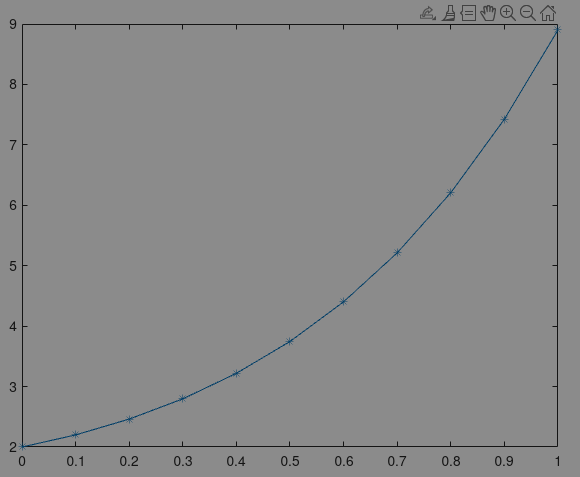
\includegraphics[width=\columnwidth]{fig7.png}
\caption{}
\label{fig:1.7}                        
  \end{figure}

\underline{RK 2 method}
\begin{lstlisting}
%RK 2 Method
clear all;
close all;
format short 
h=0.1;
x=0:h:1;
N=length(x);
y(1)=2;
f=@(x,y) y-y*x^2+2*x*y;
for i=1:N-1;
   k1=h*(f(x(i),y(i)));
   k2=h*(f((x(i)+(1/2)),(y(i)+(k1/2))));
   y(i+1)=(y(i))+h*(1/2)*(k1+k2) 
end
plot(x,y,'-*')
\end{lstlisting}
\textbf{Result:}
\begin{lstlisting}
y = 2.0000    2.0284    2.0602    2.0952    2.1331    2.1736    2.2163    2.2607    2.3066    2.3534    2.4006
\end{lstlisting}
\textbf{Figure:}
\begin{figure}[H]                                 
	  \centering                          
	  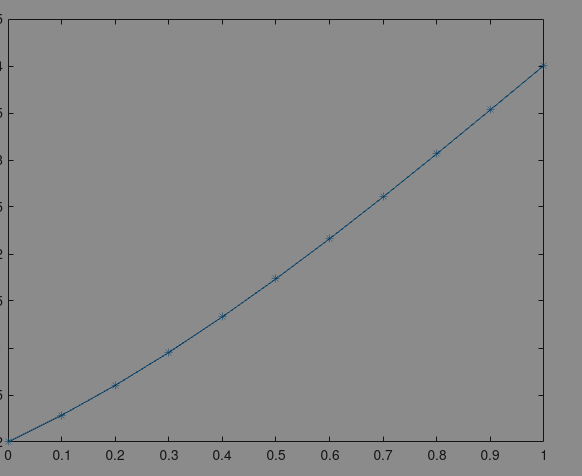
\includegraphics[width=\columnwidth]{fig8.png}
\caption{}
\label{fig:1.8}                        
  \end{figure}


    \end{enumerate}
\end{document}
